\documentclass[]{article}
\usepackage{enumitem}
\usepackage{graphicx}

\begin{document}

\textbf{APS Homework 3: Greedy Method and Iterative Improvement}

\medskip
\textbf{Problem 1: Making change}

You need to pay $n$ cents using only pennies, nickels, dimes, and quarters.
Describe an algorithm that finds a \textit{smallest} set of coins of value
exactly $n$.

\textit{Yes this is the same problem as last week only with different denominations.
Your solution however should not be the same: there's a simpler algorithm this time.}
% As always you must justify your answer; make sure that your justification would
% NOT also justify a greedy algorithm for last week's version since, as we saw in
% class, the greedy algorithm doesn't work there.

\medskip
\textbf{Problem 2: Efficient Knight}

A knight starts at the upper left of a $100 \times 100$ chessboard. What is the
fewest number of moves needed to reach the bottom right corner?

\textit{Chess rules reminder: a knight moves in an L shape with segments of lengths 2 and 1. One such L is shown
below, as are all 8 spaces the knight can move to.}

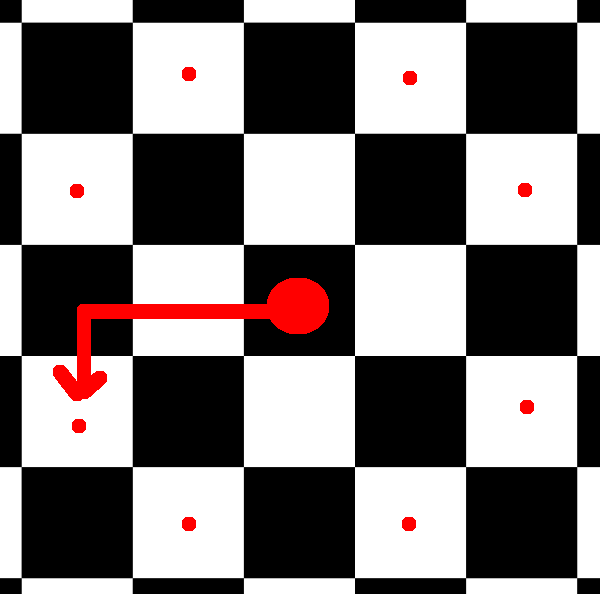
\includegraphics[scale=.2,angle=90]{knight}

\medskip
\textbf{Problem 3: Parliament Pacification}

In a parliament, each member has at most three enemies. (We assume that enmity
is always mutual.) Describe an algorithm which divides the parliament into two
chambers so that no parliamentarian has more than one enemy in their chamber.

\end{document}
